\chapter{Conclusioni}\label{ch:conclusioni}
\section{Cosa ha funzionato bene}
Il lavoro che è stato descritto in questo elaborato di tesi può essere ritenuto soddisfacente.
\\Avendo infatti come punto di partenza il \textit{paper} \cite{soccerNet} in cui venivano effettuati esperimenti analoghi a quelli effettuati da me nel mio elaborato di tesi, sono riuscito mediante l'uso di reti neurali ricorrenti ad ottenere, nel task di classificazione, risultati persino migliori.
\\In tale task infatti siamo passati da una mAP del\textbf{ 67.8\%}, ottenuta nel sopracitato \textit{paper} grazie al metodo di pooling \textbf{netVLAD}, ad una mAP del \textbf{79.7\%} ottenuta grazie all'utilizzo di \textbf{reti neurali ricorrenti}.
\\Successivamente ci siamo spinti oltre, infatti siamo passati dal task di \textbf{classificazione} a quello di \textbf{localizzazione}, questo è stato possibile grazie ad un elaborazione del dataset con un meccanismo di \textit{sliding windows}.
\\Infine è stata inoltre descritta la procedura di generazione degli highlights, la quale, utilizzando la rete neurale addestrata nel task di classificazione, ha ottenuto nel task di \textbf{spotting} un \textbf{average-F1 score} del \textbf{83.5\%}
\section{Cosa ha funzionato meno bene}
\subsection{Data Augmentation}
Durante la fase di training, per cercare di ridurre gli effetti negativi dovuti al dataset fortemente sbilanciato, si è provato a usare una tecnica di \textbf{Data Augmentation}.
\\La nostra applicazione di tale tecnica è stata utilizzata per moltiplicare i campioni di ogni evento; questo è stato possibile anche in questa situazione mediante un meccanismo di \textbf{sliding-windows}.
\\Questi ulteriori campioni sono stati aggiunti poi al dataset, aiutando a risolvere lo sbilanciamento di quest'ultimo.
\\I risultati ottenuti applicando questa tecnica non sono stati tuttavia soddisfacenti, infatti le prestazioni della rete neurale si sono rivelate peggiori rispetto al modello che non ha fatto uso di \textbf{Data Augmentation}.
\subsection{Malfunzionamenti}
La rete neurale da me sviluppata non è ovviamente \textbf{immune} da \textbf{errori}, in particolare, come evidenziato dai risultati ottenuti sia nel task di localizzazione che in quello di classificazione, l'azione che viene identificata con risultati peggiori è quella che corrisponde all'estrazione di un cartellino.
\\Nella figura \textbf{\ref{figure : fakecard}} abbiamo un esempio di tale \textbf{malfunzionamento}, infatti in tale figura vediamo come l'inquadratura \textbf{in primo piano} dell'arbitro induca la nostra rete neurale a pensare che sia stato estratto un \textbf{cartellino}, quando invece il giocatore è stato richiamato solo \textbf{verbalmente}.
\begin{figure}[H]
\centering
\caption{Visualizzazione di un cartellino non correttamente predetto}
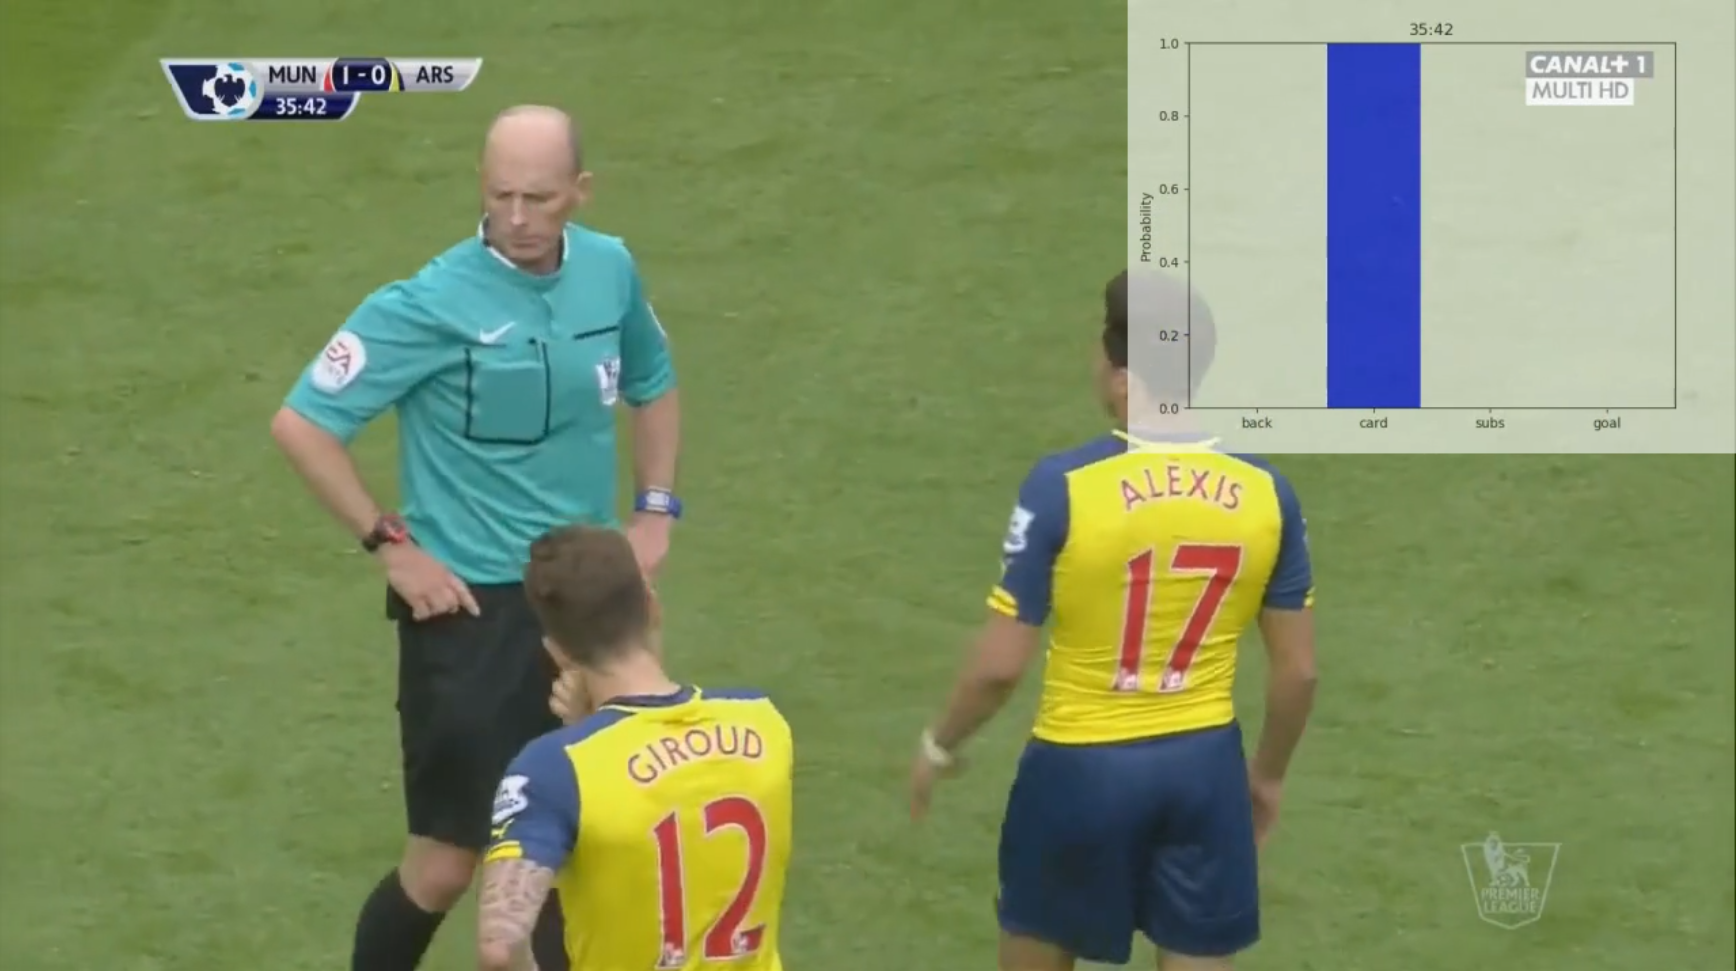
\includegraphics[width=\linewidth]{img/fakecardHQ.png}
\label{figure : fakecard}
\end{figure}
\section{Sviluppi futuri}
La naturale evoluzione di questo elaborato di tesi è quella di cercare di individuare \textbf{altre} tipologie di azioni oltre alle tre già prese in considerazione, ad esempio si potrebbero ricercare \textbf{tiri in porta}, \textbf{calci d'angolo} o \textbf{calci di rigore}.
\\Inoltre come citato nel \textit{paper} \citep{soccerNet}, nell'estrazione delle features non è stato preso in considerazione l'audio, presente invece nei video originali.
\\Indubbiamente esso aggiunge \textbf{informazioni significative} e potrebbe essere d'aiuto ai nostri scopi, tuttavia come ben sappiamo l'audio non è sempre strettamente collegato a ciò che accade in campo, ma dipende da altri fattori quali: squadra di casa, momento della partita, affluenza di pubblico allo stadio.
\\Questi fattori potrebbero \textit{confondere} la rete neurale, portando ad un peggioramento delle prestazioni.
\\Rimane impossibile quindi esprimersi a \textbf{priori} su un possibile aiuto dell'audio nell'addestramento della rete neurale.
